\documentclass{beamer} 
\usepackage{tikz}
\usepackage[all]{xy}
\usepackage{amsmath,amssymb}
\usepackage{hyperref}
\usepackage{graphicx}
\usepackage{algorithmic}
\usepackage{multirow}

\DeclareMathOperator*{\argmin}{arg\,min}
\DeclareMathOperator*{\Lik}{Lik}
\DeclareMathOperator*{\PoissonLoss}{PoissonLoss}
\DeclareMathOperator*{\Peaks}{Peaks}
\DeclareMathOperator*{\Segments}{Segments}
\DeclareMathOperator*{\argmax}{arg\,max}
\DeclareMathOperator*{\maximize}{maximize}
\DeclareMathOperator*{\minimize}{minimize}
\newcommand{\sign}{\operatorname{sign}}
\newcommand{\RR}{\mathbb R}
\newcommand{\ZZ}{\mathbb Z}
\newcommand{\NN}{\mathbb N}
\newcommand{\z}{$z = 2, 4, 3, 5, 1$} 

\newcommand{\algo}[1]{\textcolor{#1}{#1}}
\definecolor{PDPA}{HTML}{66C2A5}
\definecolor{CDPA}{HTML}{FC8D62}
\definecolor{GPDPA}{HTML}{4D4D4D}

% Set transparency of non-highlighted sections in the table of
% contents slide.
\setbeamertemplate{section in toc shaded}[default][100]
\AtBeginSection[]
{
  \setbeamercolor{section in toc}{fg=red} 
  \setbeamercolor{section in toc shaded}{fg=black} 
  \begin{frame}
    \tableofcontents[currentsection]
  \end{frame}
}

\begin{document}

\title{Cross-validation for comparing qSIP prediction models trained
  on same or other groups}

\author{
  Toby Dylan Hocking\\
  toby.hocking@nau.edu\\
  toby.hocking@r-project.org\\
}

\maketitle

\begin{frame}
  \frametitle{Machine learning predictive analysis of qSIP data}
  \begin{itemize}
  \item Inputs/features $\mathbf x\in\mathbb R^D$ is vector of TODO for D genes
    (Amplicon Sequence Variants / ASVs).
  \item Output $y\in\mathbb R$ is relative activity/growth from qSIP.
  \item Want to learn a function $f(x)=y$, using either experiment=qme
    or experiment=dim (or both). TODO Jeff what is qme/dim?
  \item Use cross-validation to quantify prediction error on held out
    test set.
  \end{itemize}
\end{frame}

% 1:       controls.between.sites       site <data.table[17225x8407]>
% 2:  control.vs.carbon.additions  treatment <data.table[60877x8407]>
% 3: controls.between.experiments experiment  <data.table[7710x8407]>
% > length(gene.names <- grep("^K", names(qsip.dt), value=TRUE))
% [1] 8380
% > for(comparison.i in 1:nrow(comparison.dt)){
% +   compare.row <- comparison.dt[comparison.i]
% +   print(compare.row$DT[[1]][, .(rows=.N), by=eval(compare.row$group.var)])
% + }
%                 site rows
% 1: glacier_forefield  767
% 2: litchfield_island 1043
% 3:                GL 3560
% 4:                MC 3120
% 5:                PJ 4317
% 6:                PP 4418
%    treatment  rows
% 1:   control 17225
% 2:         C 23214
% 3:        CN 20438
%    experiment rows
% 1:        dim 3120
% 2:        qme 4590

\begin{frame}
  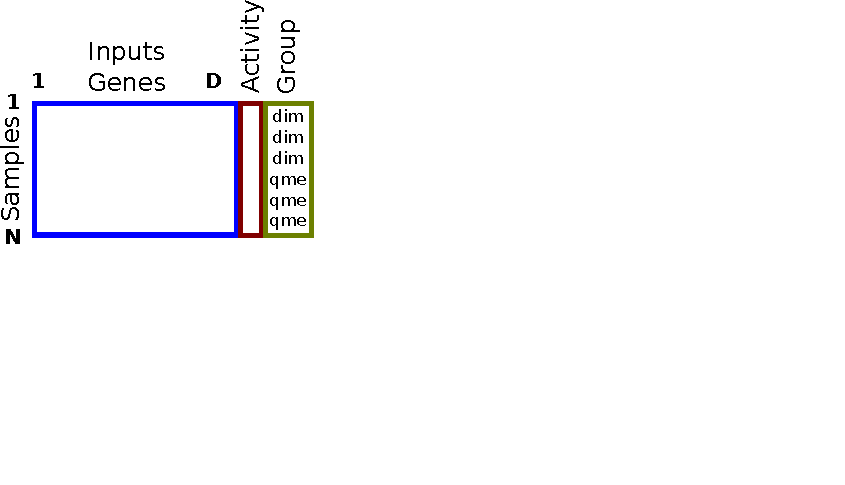
\includegraphics[width=\textwidth]{drawing-cv-same-other-1}
\end{frame}

\begin{frame}
  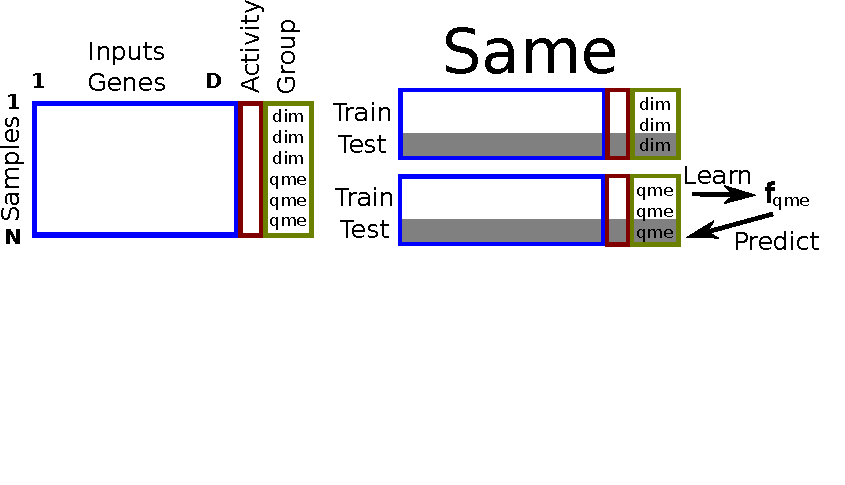
\includegraphics[width=\textwidth]{drawing-cv-same-other-2}
\end{frame}

\begin{frame}
  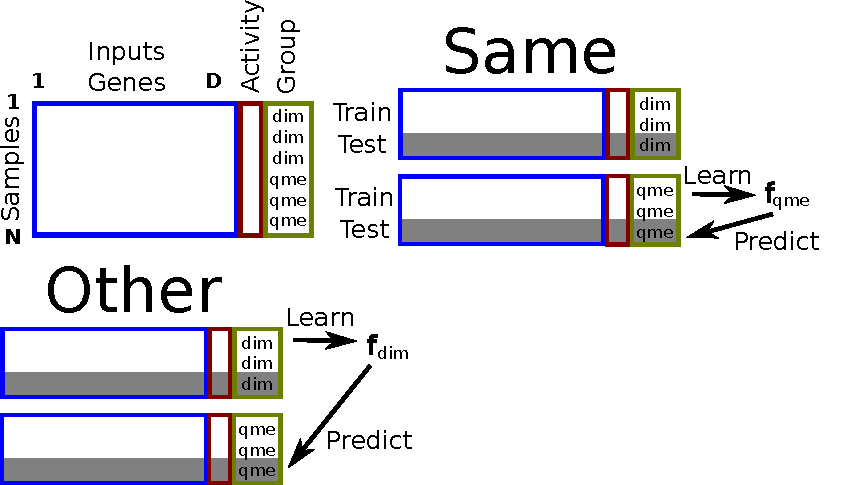
\includegraphics[width=\textwidth]{drawing-cv-same-other-3}
\end{frame}

\begin{frame}
  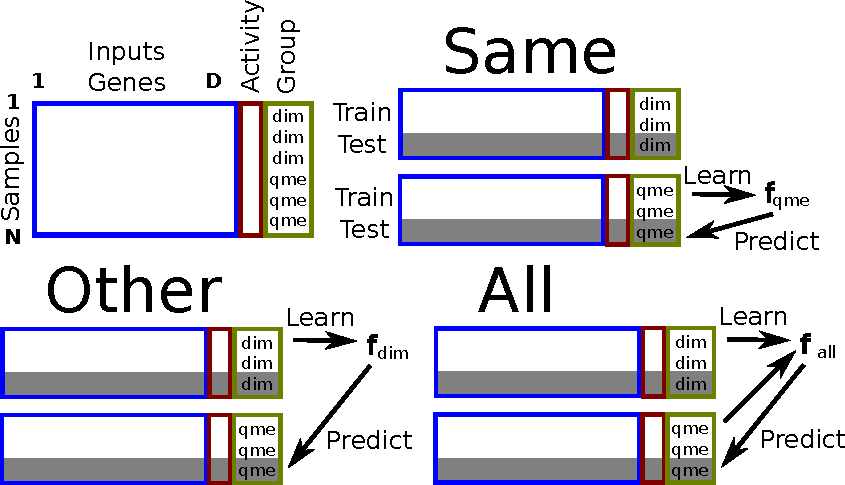
\includegraphics[width=\textwidth]{drawing-cv-same-other-4}
\end{frame}

\begin{frame}
  \frametitle{Interpreting machine learning results}
  \begin{itemize}
  \item Inputs/features $\mathbf x\in\mathbb D$ is vector of TODO for D genes
    (Amplicon Sequence Variants / ASVs).
  \item Output $y\in\mathbb R$ is relative activity/growth from qSIP.
  \item Want to learn a function $f(x)=y$, using either experiment=qme
    or experiment=dim (or both).
  \item We compare two learning algorithms
    \begin{description}
    \item[cv\_glmnet:] L1 regularized linear model (LASSO), small
      subset of important genes selected and used for prediction
      (other un-important genes are not used for prediction).
    \item[featureless] ignore all genes/features, and always predict
      mean output in train set.
    \end{description}
  \item If there is any non-trivial relationship/pattern learned
    between inputs and outputs, then \textbf{linear model should have
      smaller prediction error than featureless}.
  \item If patterns are similar in different groups/experiments (dim
    and qme), then \textbf{linear model should have similar prediction
      error, when trained on other groups/experiments}.
  \end{itemize}
\end{frame}

\begin{frame}
  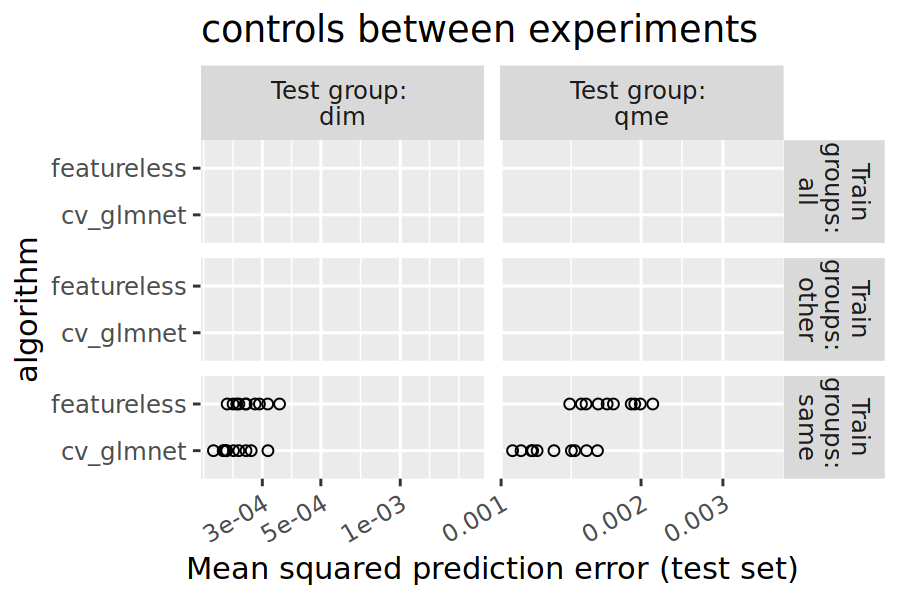
\includegraphics[width=\textwidth]{qsip_pc2_all_new-controls.between.experiments.same.png}
\end{frame}

\begin{frame}
  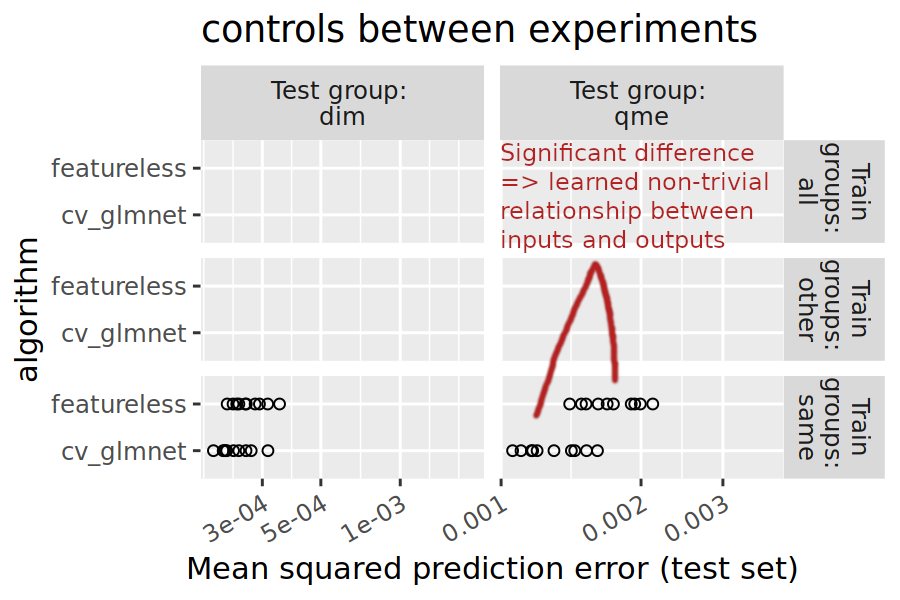
\includegraphics[width=\textwidth]{qsip_pc2_all_new-controls.between.experiments.same.ann.png}
\end{frame}

\begin{frame}
  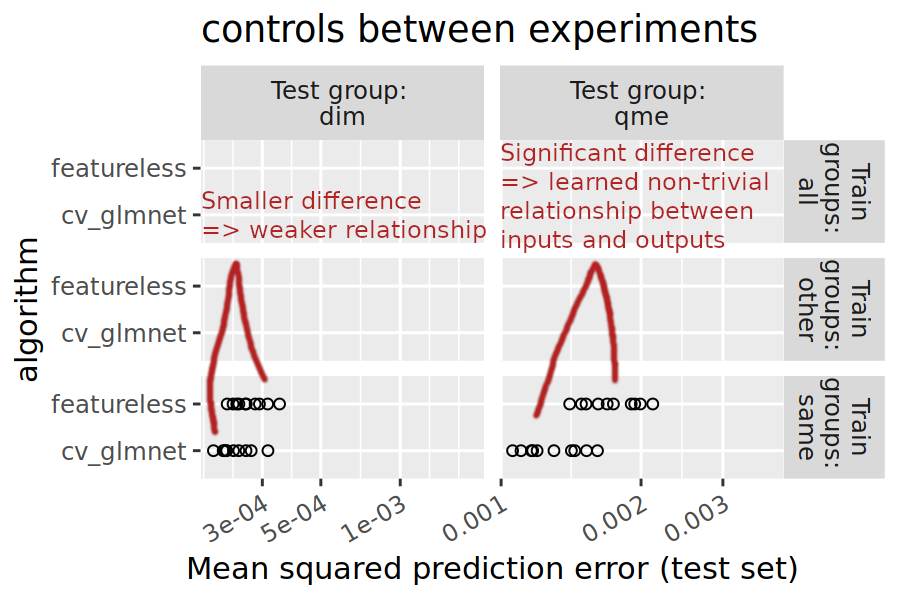
\includegraphics[width=\textwidth]{qsip_pc2_all_new-controls.between.experiments.same.ann2.png}
\end{frame}

\begin{frame}
  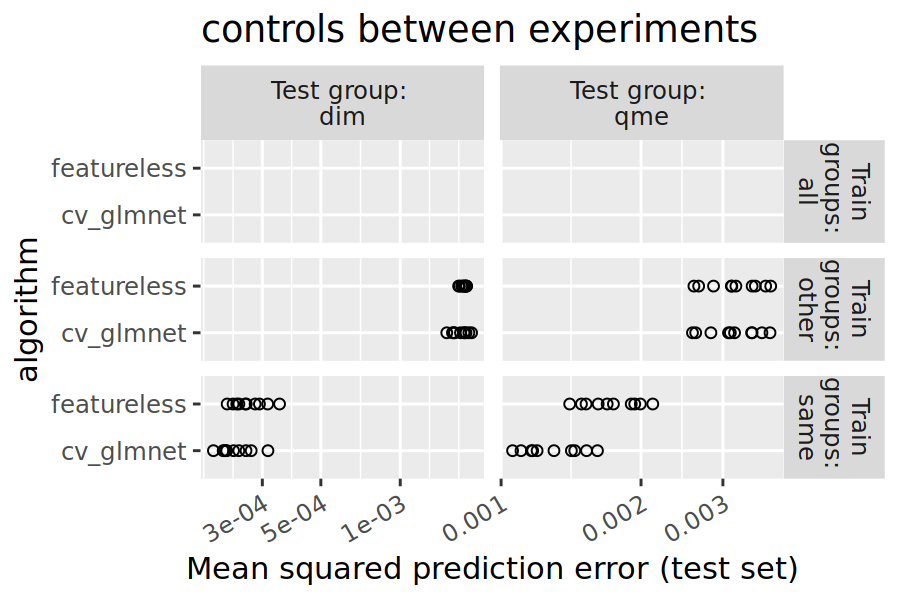
\includegraphics[width=\textwidth]{qsip_pc2_all_new-controls.between.experiments.other.png}
\end{frame}

\begin{frame}
  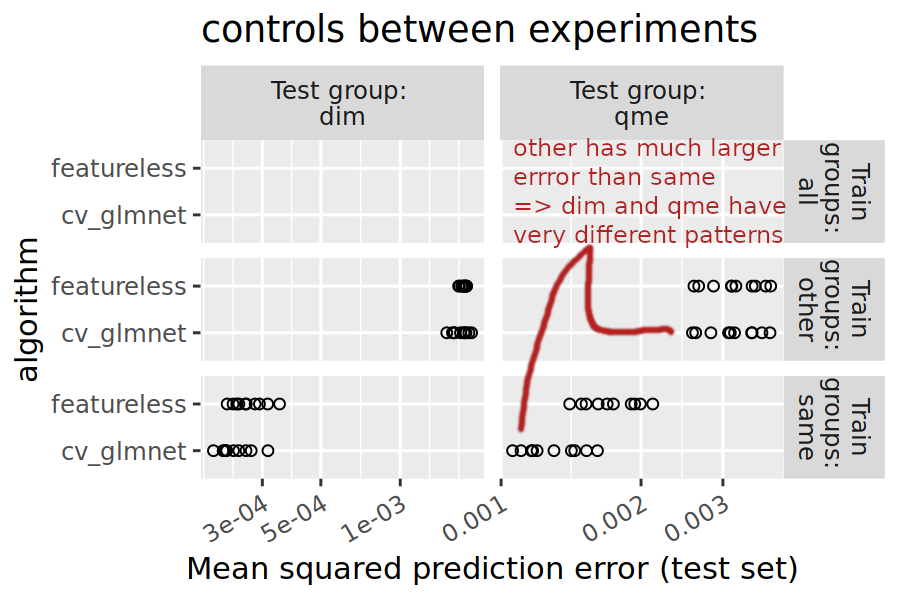
\includegraphics[width=\textwidth]{qsip_pc2_all_new-controls.between.experiments.other.ann.cpng}
\end{frame}

\begin{frame}
  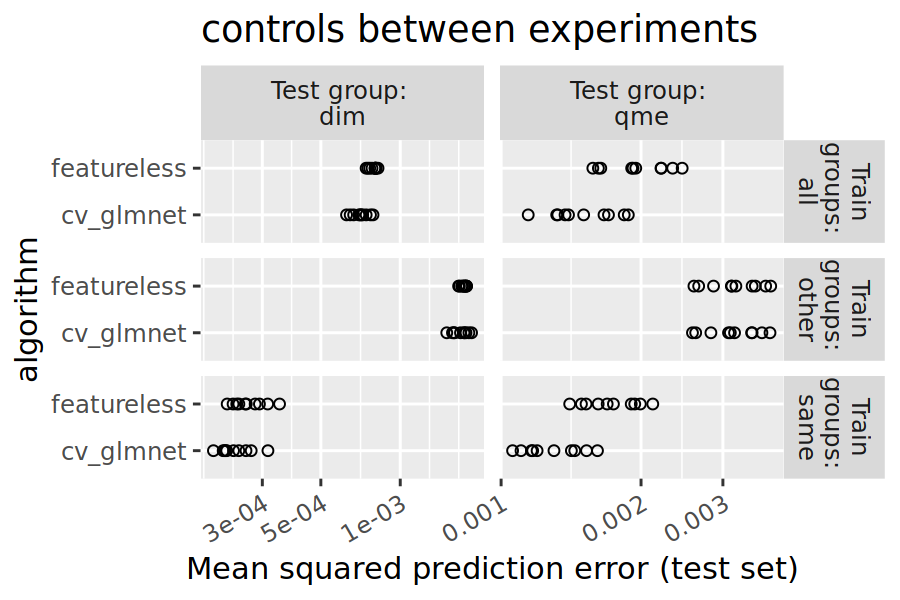
\includegraphics[width=\textwidth]{qsip_pc2_all_new-controls.between.experiments.all.png}
\end{frame}

\begin{frame}
  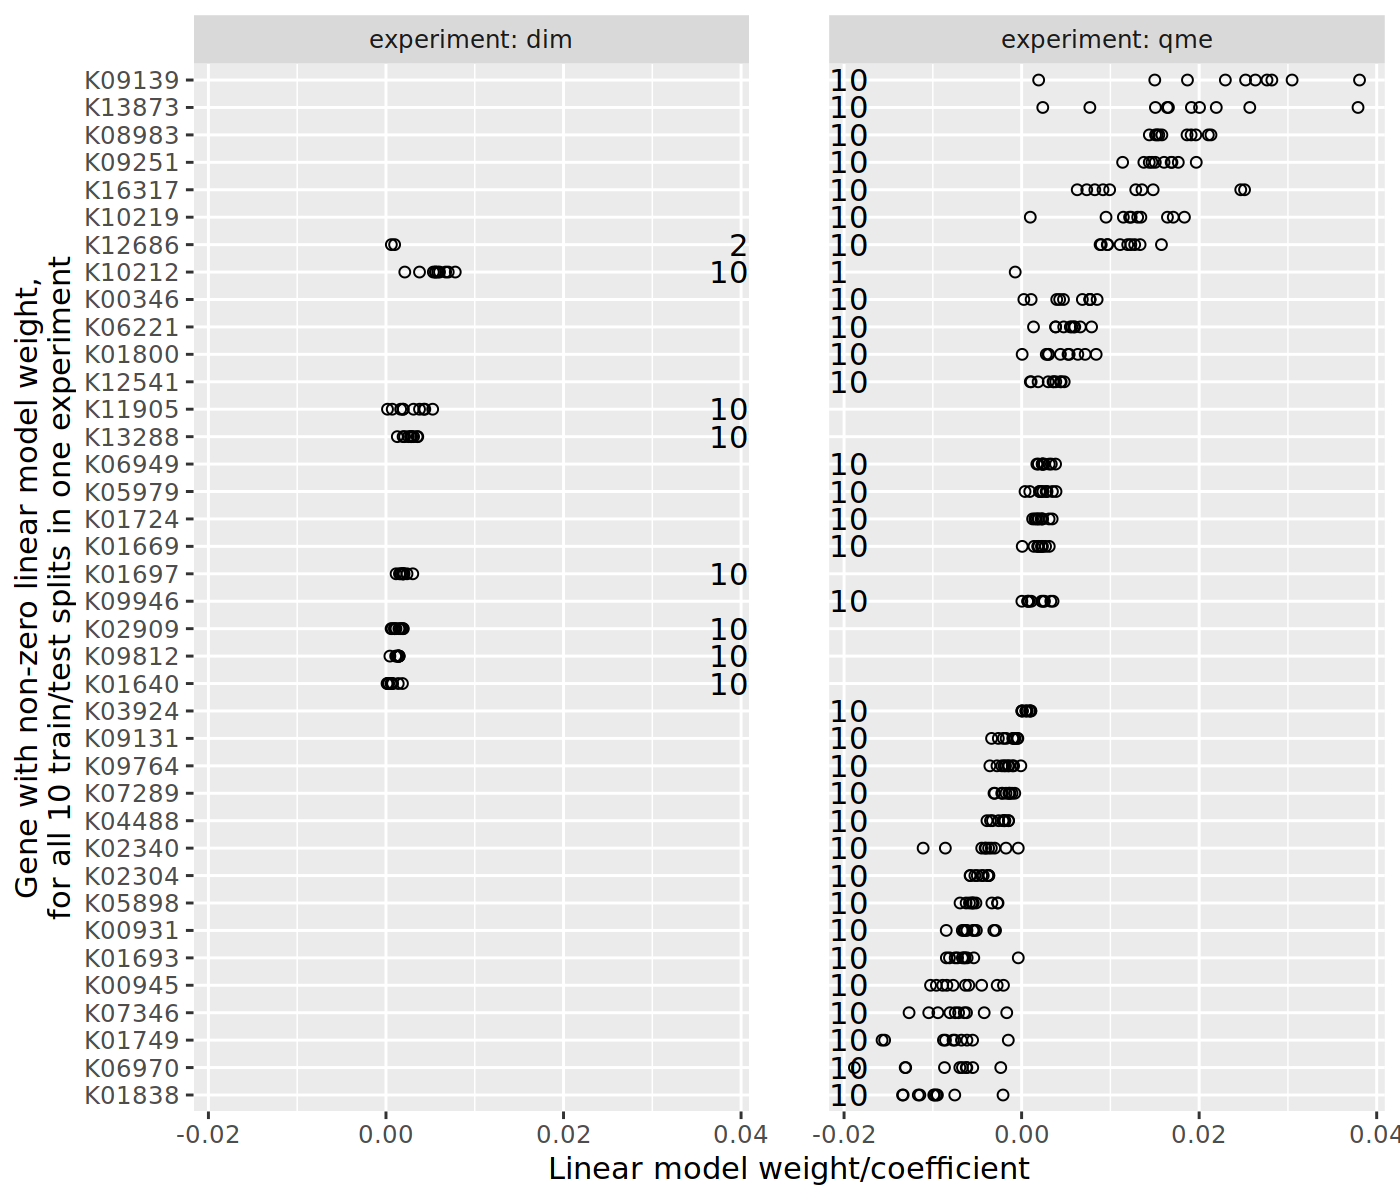
\includegraphics[width=\textwidth]{2024-01-09-qsip_pc2_all_new-controls.between.experiments.weights.png}
\end{frame}

\begin{frame}
  \frametitle{Discussion and conclusions}
  \begin{itemize}
  \item TODO
  \item Free/open-source software available: mlr3resampling R package.
  \end{itemize}
\end{frame}

\end{document}